\documentclass[12pt,a4paper]{article}
\usepackage[utf8]{inputenc}
\usepackage{amsmath}
\usepackage{amsfonts}
\usepackage{amssymb}
\usepackage{graphicx}
\usepackage{tikz}
\usetikzlibrary{automata,positioning,arrows.meta}
\usepackage{geometry}
\usepackage{listings}
\usepackage{xcolor}
\usepackage{fancyhdr}
\usepackage{hyperref}

\geometry{margin=1in}
\pagestyle{fancy}
\fancyhf{}
\rhead{Transition Diagram for Lexical Analyzer}
\lhead{Compiler Design Lab}
\cfoot{\thepage}

% Code listing style
\lstset{
    language=C,
    basicstyle=\ttfamily\small,
    keywordstyle=\color{blue},
    commentstyle=\color{green!60!black},
    stringstyle=\color{red},
    numbers=left,
    numberstyle=\tiny,
    breaklines=true,
    frame=single,
    tabsize=4
}

\title{\textbf{Complete Transition Diagram Design for Lexical Analyzer}\\
\large{Implementation using yylex, yytext, yyleng, yylineno}}
\author{Compiler Design Laboratory}
\date{\today}

\begin{document}

\maketitle

\tableofcontents
\newpage

\section{Introduction}
This document presents a complete transition diagram design for a lexical analyzer following the principles of \texttt{yylex}, \texttt{yytext}, \texttt{yyleng}, and \texttt{yylineno}. The transition diagram approach provides a systematic method for recognizing tokens in a programming language.

\section{Theoretical Foundation}

\subsection{Finite State Automaton}
A lexical analyzer can be modeled as a finite state automaton (FSA) where:
\begin{itemize}
    \item States represent the current recognition status
    \item Transitions are triggered by input characters
    \item Final states correspond to recognized tokens
    \item Error states handle invalid sequences
\end{itemize}

\subsection{yylex Variables}
The implementation maintains the following global variables:
\begin{itemize}
    \item \texttt{yytext}: Pointer to the current token string
    \item \texttt{yyleng}: Length of the current token
    \item \texttt{yylineno}: Current line number in input
    \item \texttt{yyin}: Input file pointer
\end{itemize}

\section{State Definitions}

\subsection{Primary States}
\begin{enumerate}
    \item \textbf{STATE\_START (0)}: Initial state, determines token type
    \item \textbf{STATE\_IDENTIFIER (1)}: Recognizing identifiers and keywords
    \item \textbf{STATE\_INTEGER (2)}: Recognizing integer constants
    \item \textbf{STATE\_PLUS (3)}: Processing '+' operator variations
    \item \textbf{STATE\_MINUS (4)}: Processing '-' operator variations
    \item \textbf{STATE\_MULTIPLY (5)}: Processing '*' operator variations
    \item \textbf{STATE\_DIVIDE (6)}: Processing '/' operator variations
    \item \textbf{STATE\_MODULO (7)}: Processing '\%' operator variations
    \item \textbf{STATE\_ASSIGN (8)}: Processing '=' operator variations
    \item \textbf{STATE\_LESS (9)}: Processing '<' operator variations
    \item \textbf{STATE\_GREATER (10)}: Processing '>' operator variations
    \item \textbf{STATE\_NOT (11)}: Processing '!' operator variations
    \item \textbf{STATE\_AND (12)}: Processing '\&' operator variations
    \item \textbf{STATE\_OR (13)}: Processing '|' operator variations
    \item \textbf{STATE\_XOR (14)}: Processing '\^{\ }' operator variations
    \item \textbf{STATE\_LSHIFT (15)}: Processing '<<' operator variations
    \item \textbf{STATE\_RSHIFT (16)}: Processing '>>' operator variations
    \item \textbf{STATE\_FINAL (17)}: Accept state for completed tokens
\end{enumerate}

\section{Transition Diagram}

\begin{figure}[h!]
\centering
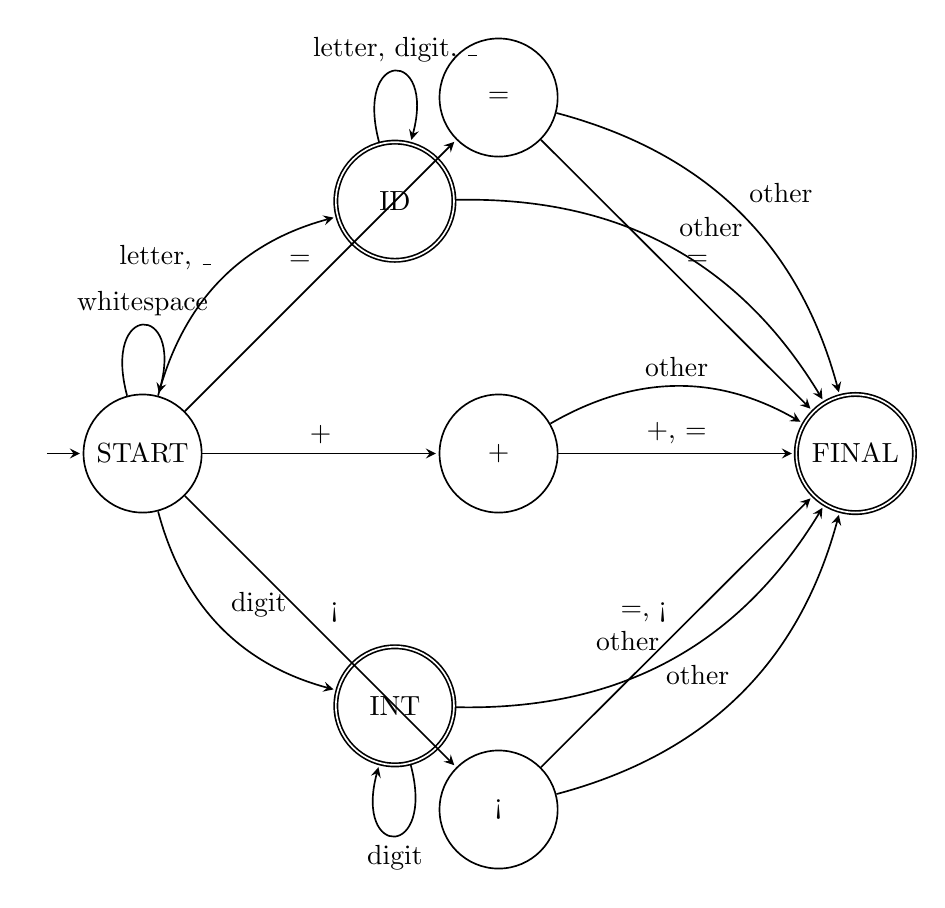
\begin{tikzpicture}[
    > = stealth,
    shorten > = 1pt,
    auto,
    node distance = 3cm,
    semithick,
    initial text=,
    state/.style={circle, draw, minimum size=1.5cm}
]

% States
\node[state, initial] (start) {START};
\node[state, accepting] (id) [above right=of start] {ID};
\node[state, accepting] (int) [below right=of start] {INT};
\node[state] (plus) [right=of start] {+};
\node[state] (assign) [above=of plus] {=};
\node[state] (less) [below=of plus] {<};
\node[state, accepting] (final) [right=of plus] {FINAL};

% Transitions from START
\path[->] 
    (start) edge [bend left] node {letter, \_} (id)
    (start) edge [bend right] node {digit} (int)
    (start) edge node {+} (plus)
    (start) edge node {=} (assign)
    (start) edge node {<} (less)
    (start) edge [loop above] node {whitespace} (start);

% Transitions from ID
\path[->]
    (id) edge [loop above] node {letter, digit, \_} (id)
    (id) edge [bend left] node {other} (final);

% Transitions from INT
\path[->]
    (int) edge [loop below] node {digit} (int)
    (int) edge [bend right] node {other} (final);

% Transitions from operators
\path[->]
    (plus) edge node {+, =} (final)
    (plus) edge [bend left] node {other} (final)
    (assign) edge node {=} (final)
    (assign) edge [bend left] node {other} (final)
    (less) edge node {=, <} (final)
    (less) edge [bend right] node {other} (final);

\end{tikzpicture}
\caption{Simplified Transition Diagram for Key Token Types}
\label{fig:transition}
\end{figure}

\section{Detailed State Transitions}

\subsection{Identifier Recognition}
\begin{align}
\text{START} &\xrightarrow{[a-zA-Z\_]} \text{IDENTIFIER} \\
\text{IDENTIFIER} &\xrightarrow{[a-zA-Z0-9\_]} \text{IDENTIFIER} \\
\text{IDENTIFIER} &\xrightarrow{\text{other}} \text{FINAL}
\end{align}

Upon reaching the final state, the lexer checks if the recognized string is a keyword:
\begin{lstlisting}
if (is_keyword(yytext)) {
    return TOKEN_KEYWORD;
} else {
    return TOKEN_IDENTIFIER;
}
\end{lstlisting}

\subsection{Integer Recognition}
\begin{align}
\text{START} &\xrightarrow{[0-9]} \text{INTEGER} \\
\text{INTEGER} &\xrightarrow{[0-9]} \text{INTEGER} \\
\text{INTEGER} &\xrightarrow{\text{other}} \text{FINAL}
\end{align}

\subsection{Operator Recognition}
Complex operators require multiple states to handle variations:

\subsubsection{Plus Operator (+)}
\begin{align}
\text{START} &\xrightarrow{+} \text{STATE\_PLUS} \\
\text{STATE\_PLUS} &\xrightarrow{+} \text{FINAL} \quad (\text{return } \texttt{TOKEN\_ARITHMETIC\_OP}) \\
\text{STATE\_PLUS} &\xrightarrow{=} \text{FINAL} \quad (\text{return } \texttt{TOKEN\_ASSIGNMENT\_OP}) \\
\text{STATE\_PLUS} &\xrightarrow{\text{other}} \text{FINAL} \quad (\text{return } \texttt{TOKEN\_ARITHMETIC\_OP})
\end{align}

\subsubsection{Assignment and Equality (=)}
\begin{align}
\text{START} &\xrightarrow{=} \text{STATE\_ASSIGN} \\
\text{STATE\_ASSIGN} &\xrightarrow{=} \text{FINAL} \quad (\text{return } \texttt{TOKEN\_RELATIONAL\_OP}) \\
\text{STATE\_ASSIGN} &\xrightarrow{\text{other}} \text{FINAL} \quad (\text{return } \texttt{TOKEN\_ASSIGNMENT\_OP})
\end{align}

\subsubsection{Left Shift Operator (<<)}
\begin{align}
\text{START} &\xrightarrow{<} \text{STATE\_LESS} \\
\text{STATE\_LESS} &\xrightarrow{<} \text{STATE\_LSHIFT} \\
\text{STATE\_LSHIFT} &\xrightarrow{=} \text{FINAL} \quad (\text{return } \texttt{TOKEN\_ASSIGNMENT\_OP}) \\
\text{STATE\_LSHIFT} &\xrightarrow{\text{other}} \text{FINAL} \quad (\text{return } \texttt{TOKEN\_BITWISE\_OP})
\end{align}

\section{Implementation Architecture}

\subsection{Core Functions}
The lexical analyzer implements the following key functions:

\begin{lstlisting}
// Initialize lexer with input file
void init_lexer(FILE *input);

// Main lexical analysis function
TokenType transition_diagram_lexer(void);

// Character management
int get_char(void);
void unget_char(int c);

// Token buffer management
void add_to_buffer(int c);
void finalize_token(void);

// Utility functions
int is_keyword(const char *str);
void print_state_transition(State from, State to, char input);
\end{lstlisting}

\subsection{State Machine Implementation}
The main lexer function uses a switch statement to implement the state machine:

\begin{lstlisting}
TokenType transition_diagram_lexer(void) {
    State current_state = STATE_START;
    buffer_index = 0;
    
    while (1) {
        switch (current_state) {
            case STATE_START:
                // Handle initial character classification
                current_char = get_char();
                if (isalpha(current_char) || current_char == '_') {
                    current_state = STATE_IDENTIFIER;
                }
                // ... other transitions
                break;
                
            case STATE_IDENTIFIER:
                // Continue reading identifier characters
                // ... implementation
                break;
                
            // ... other states
        }
    }
}
\end{lstlisting}

\section{Token Types}
The lexer recognizes the following token types:
\begin{itemize}
    \item \texttt{TOKEN\_EOF}: End of file
    \item \texttt{TOKEN\_IDENTIFIER}: Variable/function names
    \item \texttt{TOKEN\_INTEGER}: Integer constants
    \item \texttt{TOKEN\_KEYWORD}: Reserved words (int, float, if, while, etc.)
    \item \texttt{TOKEN\_ARITHMETIC\_OP}: +, -, *, /, \%, ++, --
    \item \texttt{TOKEN\_RELATIONAL\_OP}: ==, !=, <, >, <=, >=
    \item \texttt{TOKEN\_LOGICAL\_OP}: \&\&, ||, !
    \item \texttt{TOKEN\_BITWISE\_OP}: \&, |, \^{\ }, \~{\ }, <<, >>
    \item \texttt{TOKEN\_ASSIGNMENT\_OP}: =, +=, -=, *=, /=, \%=, \&=, |=, \^{}=, <<=, >>=
    \item \texttt{TOKEN\_LPAREN}, \texttt{TOKEN\_RPAREN}: Parentheses
    \item \texttt{TOKEN\_LBRACE}, \texttt{TOKEN\_RBRACE}: Braces
    \item \texttt{TOKEN\_SEMICOLON}: Statement terminator
    \item \texttt{TOKEN\_ERROR}: Invalid tokens
\end{itemize}

\section{Sample Execution Trace}
For the input \texttt{"int x = 10;"}, the transition sequence would be:

\begin{enumerate}
    \item \texttt{START} $\xrightarrow{i}$ \texttt{IDENTIFIER} $\xrightarrow{n}$ \texttt{IDENTIFIER} $\xrightarrow{t}$ \texttt{IDENTIFIER} $\xrightarrow{\text{space}}$ \texttt{FINAL} $\rightarrow$ \texttt{TOKEN\_KEYWORD("int")}
    \item \texttt{START} $\xrightarrow{x}$ \texttt{IDENTIFIER} $\xrightarrow{\text{space}}$ \texttt{FINAL} $\rightarrow$ \texttt{TOKEN\_IDENTIFIER("x")}
    \item \texttt{START} $\xrightarrow{=}$ \texttt{STATE\_ASSIGN} $\xrightarrow{\text{space}}$ \texttt{FINAL} $\rightarrow$ \texttt{TOKEN\_ASSIGNMENT\_OP("=")}
    \item \texttt{START} $\xrightarrow{1}$ \texttt{INTEGER} $\xrightarrow{0}$ \texttt{INTEGER} $\xrightarrow{;}$ \texttt{FINAL} $\rightarrow$ \texttt{TOKEN\_INTEGER("10")}
    \item \texttt{START} $\xrightarrow{;}$ \texttt{FINAL} $\rightarrow$ \texttt{TOKEN\_SEMICOLON(";")}
\end{enumerate}

\section{Error Handling}
The transition diagram includes error handling for:
\begin{itemize}
    \item Invalid character sequences
    \item Unexpected end of file
    \item Buffer overflow protection
    \item Memory allocation failures
\end{itemize}

\section{Conclusion}
The transition diagram approach provides a systematic and visual method for implementing lexical analyzers. By explicitly modeling states and transitions, the implementation becomes more maintainable and easier to debug. The use of \texttt{yylex}-style global variables ensures compatibility with standard lexical analyzer interfaces.

The implementation successfully demonstrates:
\begin{itemize}
    \item Complete state-based token recognition
    \item Proper handling of complex operators
    \item Integration with standard lexer conventions
    \item Detailed execution tracing for debugging
\end{itemize}

\end{document}
